%!TEX root = ../template.tex
%%%%%%%%%%%%%%%%%%%%%%%%%%%%%%%%%%%%%%%%%%%%%%%%%%%%%%%%%%%%%%%%%%%%
%% chapter2.tex
%% NOVA thesis document file
%%
%% Chapter with the template manual
%%%%%%%%%%%%%%%%%%%%%%%%%%%%%%%%%%%%%%%%%%%%%%%%%%%%%%%%%%%%%%%%%%%%

\typeout{NT FILE chapter2.tex}%

\chapter{Work plan}
\label{cha:work_plan}


\section{Characterization of the solution}
\label{sec:characterization_of_the_solution}

 The IOPT-Tools environment provides robust support for modeling, verifying, and generating code for individual controller sub-models using Input-Output Place-Transition (IOPT) Petri nets \cite{iopttools, barros2004, RefiningIOPT}. However, a notable challenge arises in distributed control systems, particularly those adhering to the Globally Asynchronous, Locally Synchronous (GALS) paradigm, where decomposed sub-models require inter-communication \cite{galsactd, Barrosadd}. As identified in Section~\ref{subsec:communication_gap}, the existing automatic code generation primarily focuses on the internal logic of each sub-model, necessitating manual implementation of the communication links between them. This dissertation directly addresses this gap by proposing an automated code generation tool. The core objective is to develop a mechanism that analyzes decomposed IOPT sub-models and automatically generates the necessary communication infrastructure code. This tool is envisioned to streamline the development of distributed control systems by automating the creation of efficient and reliable data exchange pathways. 
 
Figure~\ref{fig:distributed_system_example} illustrates a typical distributed control system architecture, composed of multiple micro-controllers (representing IOPT sub-models) interacting via various communication channels. This visual representation underscores the complexity and the need for automated communication management that this work addresses. Each "Micro-controller" in the figure would correspond to an independently operating IOPT sub-model, potentially residing in distinct time domains (represented conceptually by T1 and T2), and the "Communication channels" are the critical links that the proposed tool will automatically generate code for.

\begin{figure}[htbp]
  \centering
  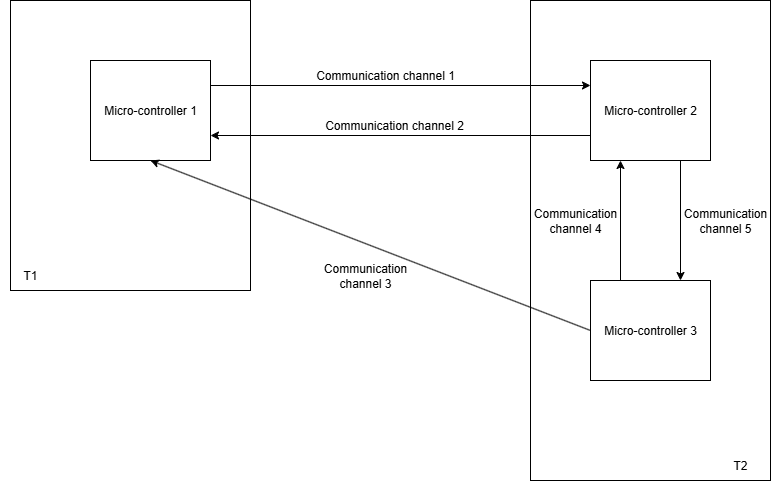
\includegraphics[width=0.8\textwidth]{solution_abstract.png}
  \caption{Example of a Distributed Control System Architecture with Communication Channels.}
  \label{fig:distributed_system_example}
\end{figure}

 
The generated code will be designed to be implemented within the communication module of each controller (Figure~\ref{fig:representation}). This targeted code placement aims to ensure seamless integration with the existing controller logic, thereby reducing development effort, minimizing manual coding errors, and enhancing the overall utility of the IOPT-Tools framework for complex distributed applications.


 \begin{figure}[htbp]
  \centering
  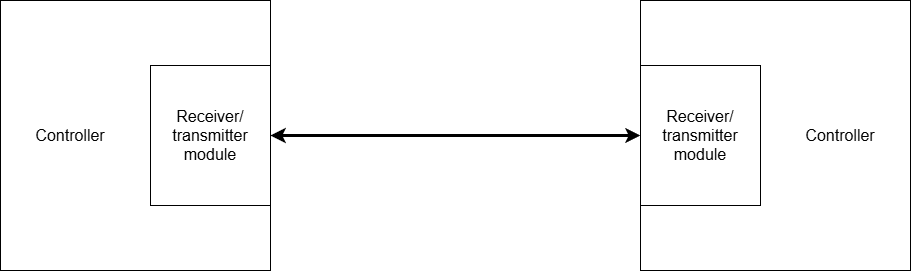
\includegraphics[width=0.6\textwidth]{Chapters/Figures/Diagrama.png}
  \caption{Solution representation.}
  \label{fig:representation}
\end{figure}
 
 
 
\section{Gant Diagram }
\label{sec:gant_diagram}

Gant diagram

\section{Task building}
\label{sec:task_building}

enumerar as tarefas que irei fazer
